\chapter{Theoretical foundations}
\section{Introduction}
In this chapter we introduce the linear fluid model of plasma wakefield acceleration and derive the equations governing the response of a plasma to an electron bunch propagating through. This model assumes that the bunch is ultra-relativistic and that the plasma density is much higher than the bunch density, which will allow us to treat the plasma response as a first order perturbation to the background density.  We also discuss the non-linear, so-called "blowout", regime which can not be treated perturbatively and is characterised by the expulsion of plasma electrons in a volume behind the bunch. The response to a laser being driven through the plasma, the so-called pondermotive force response, shares many similar features to the theory presented in this chapter but presents other issues such as dissipation and de-phasing in the plasma which will need to be address in the context of the active beam dump. For this reason the theory of laser-plasma interactions will be covered in a subsequent report. 
\section{Linear fluid model }
In this section, we derive the response of a plasma to an electron bunch by considering the plasma electrons as a fluid. We shall make the assumptions;  (i) the initial plasma is uniform and electrically neutral everywhere; (ii) the plasma ions can be considered stationary since for all plasmas the mass of the ions is much larger than the electron mass, $m_{\text{ion}}>>m_{e}$; (iii) the electron bunch is ultra-relativistic, $v/c\approx 1$, such that the density distribution of the bunch does not evolve as it interacts with the plasma; (iv) the bunch density is much less than the plasma electron density, $n_b<<n_p$.  A beam propagating through a plasma satisfying these conditions is said to be in the \textit{linear regime}. The dynamics of the plasma electrons is governed by the continuity equation
\begin{equation}
\frac{\partial n_p}{\partial t}=-\mathbf{\nabla}\cdot (n_p\vec{v}_p)
\end{equation}
where $n_p$ is the plasma electron density density and $\vec{v}_p$ the plasma fluid velocity. This simply ensures charge conservation by imposing that the plasma electron density change in a given volume is due to plasma electrons flowing in or out. The evolution of the electromagnetic fields in the plasma is governed by Maxwell's laws:
\begin{align}
\label{Maxwell1}
&\boldsymbol{\nabla}\cdot \vec{E}=4\pi \rho\\
&\boldsymbol{\nabla}\cdot \vec{B}=0\\
&\boldsymbol{\nabla}\times \vec{E}=-\frac{1}{c}\frac{\partial \vec{B}}{\partial t} \\
&\boldsymbol{\nabla}\times \vec{B}=\frac{4\pi}{c}\vec{J}+\frac{1}{c}\frac{\partial \vec{B}}{\partial t}
\label{Maxwell4}
\end{align}
which in term determine the response of the plasma fluid through the Lorentz force law:
\begin{equation}
m_e\frac{\partial n_p\vec{v}_p}{\partial t}=en_p\left(\vec{E}+\frac{\vec{v}_p\times \vec{B}}{c}\right)~.
\end{equation}
We now make use of assumption (iv)
which allows us to treat the plasma response to a particle beam perturbatively such that  $n_p=n_0+n_1$, where $n_0$ is the unperturbed uniform electron density and $n_1\ll n_0$ is the perturbation from interacting with the electron bunch. This perturbation also requires that the change in fluid velocity upon interacting with the bunch is small, such that $v_p\ll c$. Substitution into the continuity equation yields 

%Treating the plasma response to a particle beam perturbatively we have $n(r,z,t)=n_0+n_1(r,z,t)$ where $n_0$ is the ion density and $n_1$ the plasma perturbation. We let $\vec{v}, \vec{E}, \vec{B}$ be perturbative responses to the beam. From continuity equation we have
\begin{equation}
\frac{\partial n_1}{\partial t}= -n_0\left( 1- \frac{n_1}{n_0}\right)\mathbf{\nabla}\cdot \vec{v}_p
\end{equation}
Taking the time differential and neglecting terms $\mathcal{O}(n_1/n_0)$ then gives
\begin{equation}
\frac{\partial^2 n_1}{\partial t^2}= -n_0\frac{\partial (\mathbf{\nabla}\cdot\vec{v})}{\partial t}
\label{n''}
\end{equation}
Similarly, substitution into the Lorentz force law gives to first-order
\begin{equation}
 m_e\frac{\partial \vec{v}}{\partial t}= e\vec{E}
 \label{lorentz_force_plasma}
\end{equation} %m_en_0\frac{\partial (1+n_1/n_0)\vec{v}}{\partial t}\approx en_0(1+n_1/n_0)\vec{E} \quad \Rightarrow \quad 
which, using Gauss's law, gives
\begin{equation}
\frac{\partial (\mathbf{\nabla}\cdot\vec{v})}{\partial t}= \frac{e^2}{m_e}4\pi (n_1+n_b)
\label{n''2}
\end{equation}
where $n_b$ is the charge density of the electron bunch. Equations (\ref{n''}) and (\ref{n''2}) hence give
\begin{equation}
\frac{\partial^2 n_1}{\partial t^2}+\omega_p^2n_1=-\omega_p^2n_b
\label{ndotdot}
\end{equation}
where 
\begin{equation}
\omega_p=\sqrt{\frac{4\pi e^2n_0}{m_e} }
\label{plasma_frequency}
\end{equation}
is the plasma frequency. Hence the plasma density perturbation is described by a second-order differential equation with the bunch acting as a source term. We proceed to solve this for a radially symmetric bunch by evaluating equation (\ref{ndotdot}) in a reference frame co-moving with the electron bunch \cite{Dawson1959}, where the coordinate $\xi=x-ct$ represents the position along the bunch as it travels in the $x$-direction. Doing this yields
\begin{equation}
-\frac{1}{k_p^2}\left(\frac{\partial^2 }{\partial \xi^2}+k_p^2\right)n_1\left(r,\xi \right)=n_b\left(r,\xi \right) 
\end{equation}
where $k_p=\omega_p/c$ is the wavenumber and causality demands that $n_1\left(r,\xi<0 \right)=0$. We evaluate this by finding the Green's function $G\left(\xi,\xi'\right)$, which by definition obeys 
\begin{equation}
-\frac{1}{k_p^2}\left(\frac{\partial^2 }{\partial \xi^2}+k_p^2\right)G\left(\xi,\xi'\right)=\delta\left(\xi-\xi'\right)
\label{density_greens}
\end{equation}
which gives
\begin{equation}
G\left(\xi,\xi'\right)=\left\{ \begin{array}{ll}
0 &,~ -\infty<\xi<\xi'\\
A(\xi')\sin\left(k_p\xi \right) + B(\xi')\cos\left(k_p\xi \right) &,~ \xi'<\xi<\infty
\end{array}\right.
\end{equation}
where  the constant $A(\xi')$ and $B(\xi')$ are determined by by requiring continuity at $\xi=\xi'$ and by integrating equation (\ref{density_greens}) across this same boundary. This yields 
\begin{equation}
G\left(\xi,\xi'\right)=k_p\Theta(\xi-\xi')\left(\cos(k_p\xi)\sin(k_p\xi')-\cos(k_p\xi')\sin(k_p\xi)\right)
\end{equation}
and the resulting plasma perturbation is
%\begin{equation}
%\lim_{\epsilon\to 0}\int_{\xi'-\epsilon}^{\xi'+\epsilon} \mathcal{L}_{\xi}G\left(\xi,\xi'\right)\mathrm{d}\xi=\lim_{\epsilon\to 0}\int_{\xi'-\epsilon}^{\xi'+\epsilon}\delta\left(\xi\right)\mathrm{d}\xi=1 \quad \Rightarrow \quad \lim_{\epsilon\to 0}\left[-\frac{1}{k_p^2}\frac{\partial G}{\partial \xi}\right]^{\xi'+\epsilon}_{\xi'-\epsilon}=1
%\end{equation}
%Without loss of generality we may set the arrival of the beam to be at $t=0$, such that $\xi'=0$.
\begin{equation}
\begin{aligned}
n_1\left(r,\xi \right)&=\int_{-\infty}^{\infty}G\left(\xi,\xi'\right)n_b\left(r,\xi' \right) \mathrm{d}\xi'\\
&=\int_{-\infty}^{\xi}\sin\left(k_p(\xi-\xi')\right)n_b\left(r,\xi' \right) \mathrm{d}\xi'
\end{aligned}
\label{density_perturbation}
\end{equation}
where we have used the trigonometric identify for $\sin\left(k_p(\xi-\xi'\right))$. Hence the electron bunch induces oscillatory density perturbations in the plasma with a wavelength given by $\lambda_p=2\pi/k_p$. In addition, the magnitude of these perturbation scales linearly with $n_b$, the density of the beam driver. Equation (\ref{plasma_frequency}) further shows that these perturbations scale as $n_0^(1/2)$, the square root of the plasma density. These perturbations set up electromagnetic fields in the plasma behind the beam driver. An understanding of these fields is crucial in order to design a functioning plasma wakefield experiment.
\subsection{Longitudinal Accelerating Field} 
The electric field parallel to the propagation of the beam driver is what drives particles to either accelerate or decelerate. This is called the longitudinal plasma wakefield and in this section we proceed to derive an expression for it in the linear regime considered above. 
From Maxwell's equations (\ref{Maxwell1}-\ref{Maxwell4}) it is straightforward to show that the electric field in the plasma obeys a wave equation:
\begin{equation}
\nabla^2\vec{E}-\frac{1}{c^2}\frac{\partial^2 \vec{E}}{\partial t^2}=\frac{4\pi}{c^2}\frac{\partial \vec{J}}{\partial t}+4\pi\boldsymbol{\nabla}\rho
\label{E_wave_equation}
\end{equation}
where the change in current and variations in the charge density act as source terms. Letting $\rho=\rho_b+\rho_p$ be the total charge density and $\vec{J}=\vec{J}_b+\vec{J}_p$ be the total charge current, where $b$ and $p$ denote the beam and plasma respectively, we have from equation (\ref{lorentz_force_plasma}) that 
\begin{equation}
\frac{\partial \vec{J}_p}{\partial t}=\frac{e^2 n}{m}\vec{E}
\end{equation}
Substituting this into equation (\ref{Ex_wave_equation}), together with $\vec{J}_b=c\rho_b\hat{\vec{z}}$, and taking the z-component gives
%\begin{equation}
%\left(\nabla^2-\frac{1}{c^2}\frac{\partial^2}{\partial t^2}-k_p^2\right)\vec{E}=\frac{4\pi}{c}\frac{\partial \rho_b}{\partial t}\hat{\vec{z}}+4\pi\boldsymbol{\nabla}\left(\rho_b+\rho_p\right)
%\end{equation}
\begin{equation}
\left(\nabla^2-\frac{1}{c^2}\frac{\partial^2}{\partial t^2}-k_p^2\right)E_z=\frac{4\pi}{c}\frac{\partial \rho_b}{\partial t}+4\pi\frac{\partial}{\partial z}\left(\rho_b+\rho_p\right)
\label{Ez_wave_equation}
\end{equation}
where $k_p=\omega_p/c$ is the plasma wave number and $E_z$ is the longitudinal electrical field. To solve this we write $\nabla^2=\nabla^2_{\perp}+\partial^2_z$ in  transverse and longitudinal components. Furthermore, we proceed to work in Fourier transform space, where
%\textcolor{purple}{change this to E=integral tilde E, then substitute that into the following equations, since the RHS of 2.14 is not correct, fourier transform of the derivative acting on the function is not the same as the derivative acting on the transformed function}
\begin{equation}
E_z(\xi)=\frac{1}{2\pi}\int_ {-\infty}^{\infty}\wtilde{E}_z(k)e^{ik\xi}\mathrm{d}k
\end{equation}
and similarly for $\rho_b$ and $\rho_p$. Equation (\ref{Ez_wave_equation}) now simplifies to
%\begin{equation}
%\left(\frac{\partial^2 }{\partial z^2}-\frac{1}{c^2}\frac{\partial^2 }{\partial t^2}\right)E_z(\xi)=0
%\end{equation}
%and
%\begin{equation}
%\frac{4\pi}{c}\frac{\partial {\rho}_b}{\partial t}+4\pi\frac{\partial }{\partial z}\left({\rho}_b+{\rho}_p\right)=-4\pi i k\wtilde{\rho}_b+4i k\pi\wtilde{\rho}_b+4i k\pi\wtilde{\rho}_p=4i k\pi\wtilde{\rho}_p
%\end{equation}
%which gives 
\begin{equation}
\left(\nabla^2_{\perp}-k^2_p\right)\wtilde{E}_z\left(\xi\right)=4\pi i k\wtilde{\rho}_p~,
\end{equation}
We note that the two contributions from the beam, $\vec{J}_b$ and $\rho_b$, have cancelled each other out. This is because the beam velocity was set to be ultrarelativisitc, $\beta=1$, such that the electric field witnessed by the stationary plasma electrons is purely in the radial direction \citep{Gessner2016}. The effect of the beam is however represented in the plasma modulations through equation (\ref{density_perturbation}). It is convenient to write this relationship in a compact form by taking the Fourier transform of equation (\ref{ndotdot}) to find that
%\begin{equation}
%\frac{\partial^2{\rho}_p}{\partial t^2}+\omega_p^2{\rho}_p=-\omega_p^2{\rho}_b \quad \Rightarrow\quad
%-k^2\wtilde{\rho}_p+k_p^2\wtilde{\rho}_p=-k_p^2\wtilde{\rho}_b 
%\end{equation}
%which gives 
\begin{equation}
\wtilde{\rho}_p=\frac{k_p^2}{k^2-k_p^2}\wtilde{\rho}_b~.
\end{equation}
which together with the cylindrical representation of the Laplacian
\begin{equation}
\nabla_{\perp}^2=\frac{1}{r}\frac{\partial }{\partial r}r\frac{\partial }{\partial r} +\frac{1}{r^2}\frac{\partial^2 }{\partial \phi^2} 
\end{equation}
gives
\begin{equation}
 \left(\frac{\partial^2 }{\partial r^2}+\frac{1}{r}\frac{\partial }{\partial r} -k^2_p\right)\wtilde{E}_z
=4\pi ik_p^2 \frac{k}{k^2-k_p^2}\wtilde{\rho}_b
\label{diffeq_in_transformspace}
\end{equation}
where we have assumed that the longitudinal field is radially symmetric. This is the Fourier transformed version of equation (\ref{Ez_wave_equation}), which has the advantage of the source term being a function of the Fourier transform of the beam density alone. At this point it should be noted that a setting the beam velocity to $\beta=1$ before solving this equation, as we have done here, is technically not valid...... However, the effect of this is altogether negligible in our case (calc extra term from their paper).\\
We now rewrite this equation as
\begin{equation}
\mathscr{L}\wtilde{E}_z= \wtilde{f}(r)
\end{equation}
Hence by solving this this PDE we can find $E_z$ through inverse the Fourier transform. We do this by finding its Green's function $G(\vec{r},\vec{r}')$. Working in a cylindrical coordinate system we have that the Green's function must satisfy 
\begin{equation}
\mathscr{L}G(\vec{r},\vec{r}')=\frac{1}{r}\delta(r-r')\delta(\phi-\phi')\delta(z-z')
\end{equation}
where the 3-dimensional Dirac delta function is written in cylindrical polar coordinates and defined such that $\int\delta(\vec{r}-\vec{r}')r\mathrm{d}r\mathrm{d}\phi\mathrm{d}z=1$. Since the PDE is a function of the radius we can write the Green's function as
\begin{equation}
G(\vec{r},\vec{r}')=G_r(r,r')\delta(\phi-\phi')\delta(z-z')
\end{equation}
which leads to 
\begin{equation}
\mathscr{L}G_r(r,r')=\frac{1}{r}\delta(r-r')
\label{greens_diff_eq}
\end{equation}
The left-hand side of this expression is the modified Bessel function of order zero \cite{Jackson1962}. Consequently, the Green's function is formed by linear combinations of the two modified Bessels functions of order zero, which we denote by $K_0$ and $I_0$: %\todo{Standard Bessel function with complex arguments} the linearly independent, 
\begin{equation}
G\left(r,r'\right)=\left\{ \begin{array}{ll}
A(r')(A_1 I_0(k_pr)+B_1K_0(k_pr)) &,~ 0<r<r'\\
B(r')(A_2 I_0(k_pr)+B_2K_0(k_pr))  &,~ r'<r<\infty~.
\end{array}\right.
\end{equation}
By requiring that the two parts of this expression each satisfy one of the boundary conditions we have that $B_1=A_2=0$ since $K_0(k_pr)\to \infty$ as $r\to 0$ and $I_0(k_pr)\to \infty$ as $r\to \infty$. Continuity in $G(r,r')$ at $r=r'$ further gives that 
\begin{equation}
G\left(r,r'\right)=A_0\left\{ \begin{array}{ll}
I_0(k_pr)K_0(k_pr') &,~ 0<r<r'\\
I_0(k_pr')K_0(k_pr)  &,~ r'<r<\infty
\end{array}\right.
\end{equation}
where $A_0$ is a constant of proportionality that we find by integrating %$\mathscr{L}G(r,r')=\delta(r-r')/r$ 
equation (\ref{greens_diff_eq}) for $r\in\left[r'-\epsilon, r'+\epsilon \right]$. This expression needs to be satisfied for all $\epsilon$, including the limit as $\epsilon\to 0$, such that
%\begin{equation}
 %\lim_{\epsilon\to 0}\int_{r'-\epsilon}^{r'+\epsilon}\left(\frac{\partial^2 G}{\partial r^2}+\frac{1}{r}\frac{\partial G}{\partial r} -k^2_pG\right)\mathrm{d}r= \lim_{\epsilon\to 0}\int_{r'-\epsilon}^{r'+\epsilon}\frac{1}{r}\delta(r-r')\mathrm{d}r
 %\end{equation}
\begin{equation}
\lim_{\epsilon\to 0}\int_{r'-\epsilon}^{r'+\epsilon}\mathscr{L}G_r(r,r')\mathrm{d}r= \lim_{\epsilon\to 0}\int_{r'-\epsilon}^{r'+\epsilon}\frac{1}{r}\delta(r-r')\mathrm{d}r
 \end{equation}
 which gives  %\lim_{\epsilon\to 0}\Big[\frac{1}{k_p}\frac{\partial G}{\partial r} \Big]_{z-\epsilon}^{z+\epsilon}=
 \begin{equation}
 \frac{A_0}{k_p} \left.\left(I_0(k_pr')\frac{\partial K_0(k_pr)}{\partial r}-\frac{\partial I_0(k_pr)}{\partial r}K_0(k_pr')\right)\right|_{r=r'} =\frac{1}{r'}~.
 \end{equation}
This equality must hold for all finite values of $r'$. Hence, following an approach by Jackson \citep{Jackson1962}, we evaluate this expression for $k_pr'\gg 1$, where $I_0$ and $K_0$ take the limiting forms: 
\begin{equation}
I_0(k_pr')\to \frac{1}{\sqrt{2\pi k_pr'}}e^{k_pr'} \quad \text{and} \quad K_0(k_pr')\to \sqrt{\frac{\pi}{2k_pr'}}e^{-k_pr'}
\end{equation}
which implies that $A_0=-1$. The Green's function can then be written, using the Heavieside step function $\Theta(r)$, as %\textcolor{purple}{Here Gessner gets $A=4\pi$ because of Jackson but I don't see why.} 
\begin{equation}
G\left(r,r'\right)=- I_0(k_pr)K_0(k_pr')\Theta(r'-r)-I_0(k_pr')K_0(k_pr)\Theta(r-r')~.
\end{equation}
We can thus find $\wtilde{E}_z$ from 
\begin{equation}
\wtilde{E}_z(r,k)=\int_{0}^{\infty}G\left(r,r'\right)f(r',k)r'\mathrm{d}r'
\end{equation}
and then perform an inverse Fourier transform to find 
%\begin{equation}
%E_z(r,\xi)=\frac{1}{2\pi}\int_ {-\infty}^{\infty}\wtilde{E}_z\left(r,k\right)e^{ik\xi}\mathrm{d}\xi
%\end{equation}
%Doing this yields 
\begin{align}
E_z(r,\xi)&=-{2ik_p^2}\int_{-\infty}^{\infty}\frac{ke^{ik\xi}}{k^2-k_p^2}\mathrm{d}k\int_0^{\infty}\left( I_0(k_pr)K_0(k_pr')\Theta(r'-r)+I_0(k_pr')K_0(k_pr)\Theta(r-r') \right)\wtilde{\rho}_b(r')r'\mathrm{d}r'
\label{e_z}
\end{align}
%For a known beam distribution $\rho_b(r,\xi)$ (add $\xi$ in all previous expressions?) this expression can be used to compute the resulting longitudinal electric field. We shall now proceed by calculating this for a bi-Gaussian bunch distribution. To do this, we could compute the electric field from the Green's function directly and then carrying out the inverse Fourier transform, or we could choose to first compute the field due to a point-particle and then convolving it with the bi-Gaussian distribution. We proceed by doing the latter by following the approach of Dawson \cite{Katsouleas1987} ; we choose a charge distribution with radial symmetry and a delta function in the $z$-direction to match our Green's function.
For a known beam distribution $\rho_b(r,\xi)$ this expression can be used to compute the resulting longitudinal electric field. Of particular interest to us is the field induced by the propagation of a bi-Gaussian electron bunch. To compute this we follow an approach by Dawson \cite{Katsouleas1987} and first evaluate the field due to a point-particle and then convolve it with our bi-Gaussian driver. We choose a radially symmetric charge distribution ${\rho}_{0}$ with a delta function in the $\xi$ direction so as to match our Green's function:
\begin{align}
{\rho}_{0}(r,\xi)=\frac{e}{2\pi r}\delta(r-r')\delta(\xi) %\quad \Rightarrow\quad  \wtilde{\rho}_{b_0}(r,k)=\int_ {-\infty}^{\infty}\rho_b(r,\xi)e^{-ik\xi}\mathrm{d}\xi=\frac{e}{2\pi r}\delta(r-r')
\end{align}
Substituting the Fourier transform of this into equation (\ref{e_z}) and performing a contour integrating in k-space yields 
\begin{equation}
E_z(r,\xi)=-2ek_p^2\cos(k_p\xi)G\left(r,r'\right)\Theta(\xi)~,
\label{singe-particle-wake}
\end{equation}
where $\Theta(\xi)$ ensures causality is preserved. This is the so called single-particle wake function \cite{Katsouleas1987}. The longitudinal electric field resulting from an arbitrary radially-symmetric source distribution $n_b(r,\xi)$ is now given by convolving the source by the single-particle wake function:
\begin{align}
E_z(r,\xi)&=-2ek_p^2\int_0^{2\pi}\mathrm{d}\phi  \int_{-\infty}^{\infty} \cos(k_p(\xi-\xi'))\Theta(\xi-\xi')\mathrm{d}\xi' \int_{0}^{\infty}G\left(r,r'\right) n_b(r',\xi')r'\mathrm{d}r'\\
&=-4\pi e k_p^2 \int_{-\infty}^{\xi} \cos(k_p(\xi-\xi'))\mathrm{d}\xi' \int_{0}^{\infty}G\left(r,r'\right) n_b(r',\xi')r'\mathrm{d}r'
\end{align}
%\begin{equation}
%\wtilde{E}_z(r,k)=-2eik_p^2\frac{k}{k^2-k_p2}G\left(r,r'\right)
%\end{equation}
%which satisfies (\ref{diffeq_in_transformspace}), as can be shown by integrating across the discontinuity and taking the limit to zero, and then gives
%\textcolor{red}{But my Green's function has a $A=-1$ as constant and not $A=4\pi$ as Bonatto and Gessner}\\
The electric force is thus $F_z(r,\xi)=-eE_z(r,\xi)$. To compare with simulations and experiments we now choose to convert from CGS to SI units by having $e^{\text{CGS}}\to e^{SI}/\sqrt{4\pi\epsilon_0}$. The electric force in SI units (J/m) is thus
\begin{equation}
F_z(r,\xi)=\frac{e^2 k_p^2}{\epsilon_0} \int_{-\infty}^{\xi} \cos(k_p(\xi-\xi'))\mathrm{d}\xi' \int_{0}^{\infty}G\left(r,r'\right) n_b(r',\xi')r'\mathrm{d}r'
\label{longitudinalforce}
\end{equation}
To further understand this electric field and its relation to the electron beam we will calculate this numerically for a bi-gaussian bunch with a density of the form
\begin{equation}
\rho_b(r,\xi)=\frac{N_b}{(2\pi)^{3/2}\sigma_r^2\sigma_{\xi}}e^{-\xi/(2\sigma_{\xi}^2)-r/(2\sigma_{r}^2)}
\label{bigaussian}
\end{equation}
where $N_b$ is the number of electrons in the bunch and $\sigma_{\xi}$ and $\sigma_r$ are the standard deviation of the bunch in the longitudinal and transverse direction. We choose the plasma density $n_p=100n_b$ to ensure that the electron beam is in the linear regime. At this point, to show that the linear fluid model is valid, we also compare this calculation to a simulation of the same situation. The way in which this simulation has been done is covered extensively in chapter 3. The result of this is shown in figure \ref{theory_vs_simulation}. We note that the theoretical calculations and the simulations are indeed in good agreement, with the model predicting both the amplitude and the wavelength of the induced electric fields in the plasma. We further note that the electric field is positive along the bunch, which implies that the force on the electron bunch is opposite the direction of travel. Hence the electron bunch in this case should lose energy and slow down. This might at first sight appear unsuprising, since if the bunch moved through a solid material it would loose energy as well, and as the bunch moves through the plasma it displaces electrons which transfers kinetic energy to the plasma. The surprise here however is the uneven way in which the plasma electrons rearrange themselves. Each electron displaces plasma electrons, and each electron transfers a small amount of energy to the plasma electrons, the plasma electrons arrange themselves in such a way as to collective create a large electric field in the middle of the bunch. So even though each electron transfers some energy kinetically, the ones in the middle will lose a lot more energy through this decelerating  electric field which all the electrons in the bunch has contributed to setting up. This is particularly evident for the head of the bunch, which according to both the theory and the simulations should experience a zero value electric field and therefore only loose energy through scattering mechanisms, which is entirely negligible compared to the electric field. Hence, in contrast to propagation through solid matter we expect the head of the bunch to maintain its energy when moving through a plasma.\\
 We may furthermore predict that this method can not fully deplete the energy of the beam on its own. For, assuming that the electric field maintains its form as the beam propagates, as soon as particles lose enough energy and fall behind the rest of the bunch, they will end up in a region of positive electric field and subsequently get reaccelerated. One method for dealing with this was described in chapter 1, whereby Wu et al. simulated the use of foils to prevent particles reaching the reacceleration region. The other method, proposed by Hanahoe et al. was to let the beam propagate through an increasing plasma density. Although this method has not been simulated so far, if the proposed experiment at FLASHForward at DESY in 2019 include the possibility to test this proposal this method will need to be explored further in the upcoming report. This method utilizes the transverse wakefields and we cover them below for completeness. 
%For this reason this is referred to as collective deceleration. 
\begin{figure}
\centering
\includegraphics[width=0.95\textwidth]{longitudinal_2d_plot}
\label{transverse_plot}
\caption{•}
\end{figure}
\begin{figure}
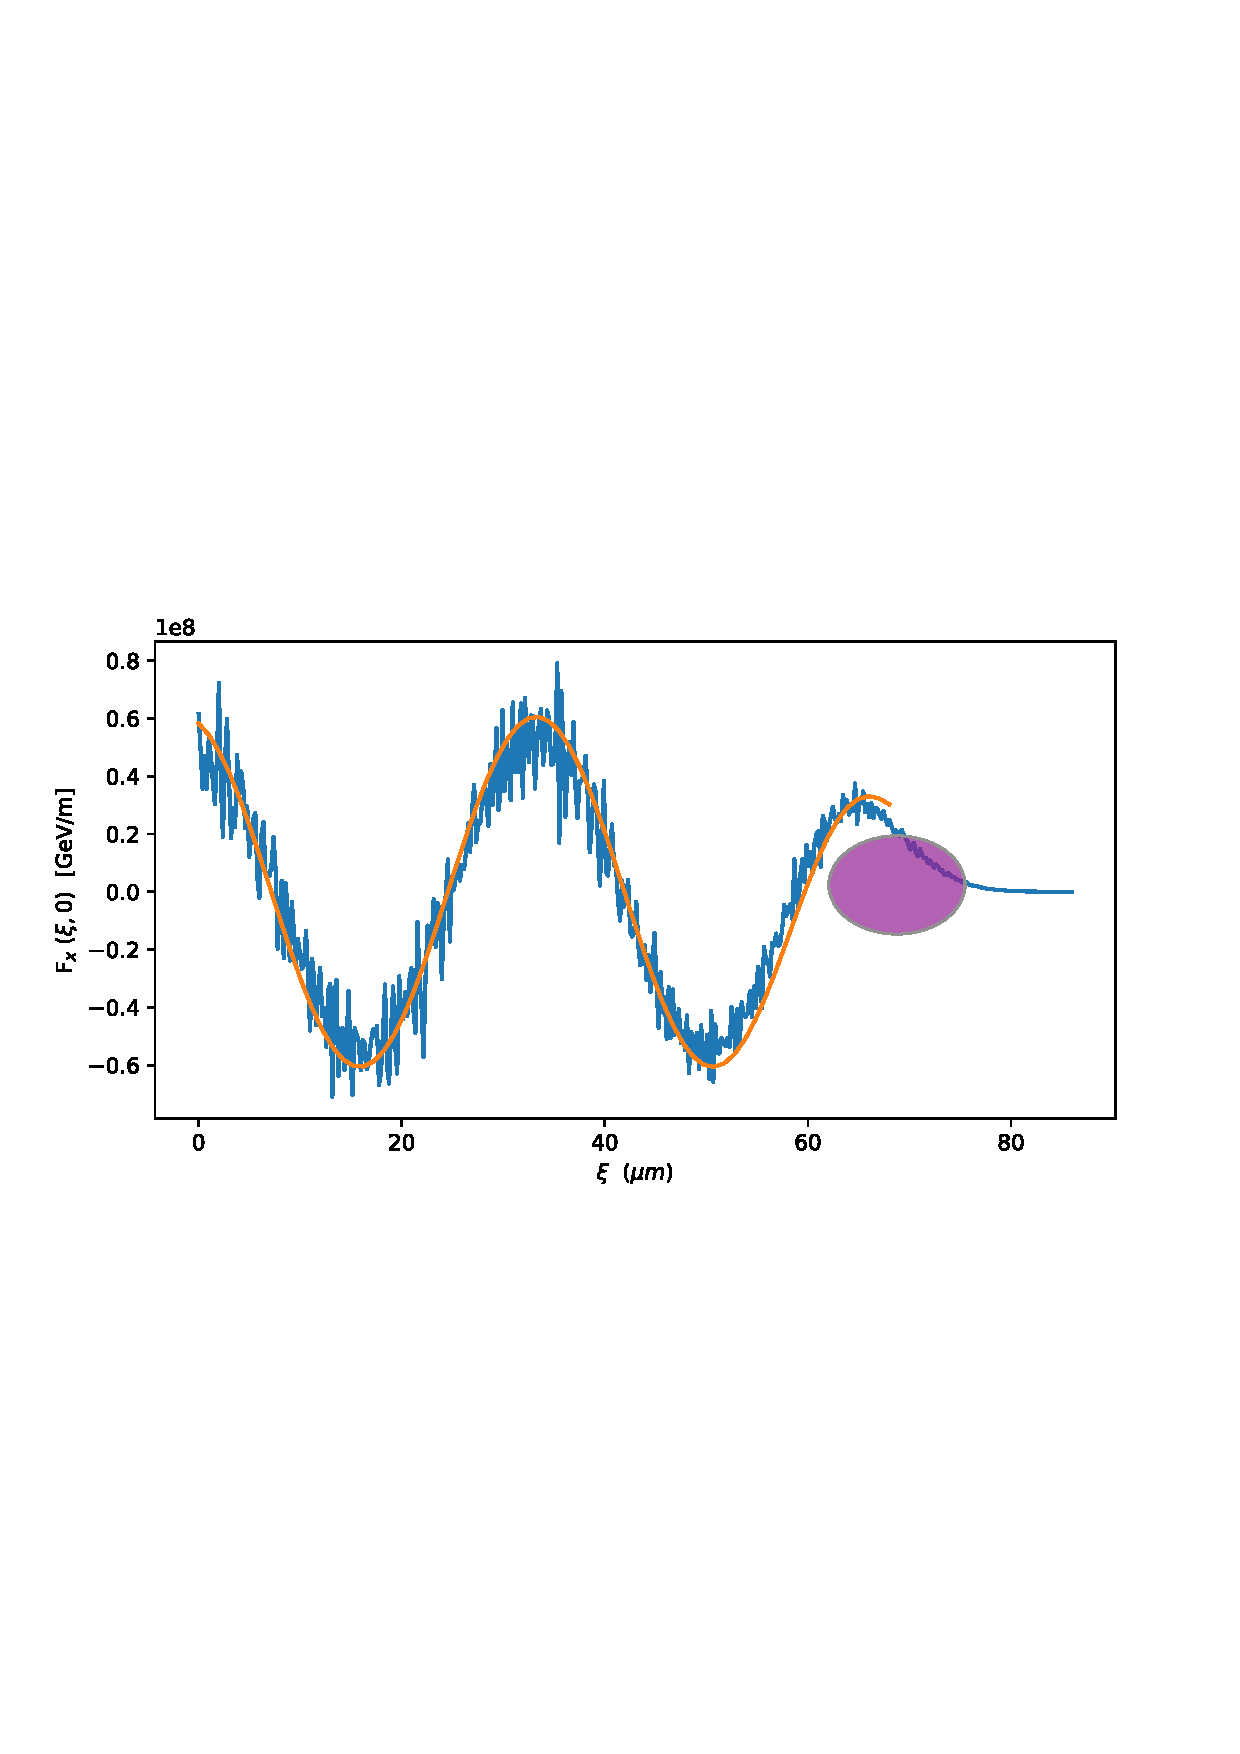
\includegraphics[width=\textwidth]{linear_SimVsTheory_bunch.pdf}
\caption{Simulation vs. theory for linear regime with $n_p/n_b=100$. }
\label{theory_vs_simulation}
\end{figure}
\subsection{Transverse Field} 
An ultrarelativisitic electron bunch will be highly contracted in the direction of propagation relative to the plasma electrons in the 'lab' frame. Assuming $\beta=1$ as before the electric field due to the bunch is purely radial, $E_r$. In addition, the magnetic field due to the charge is azimuthal, $B_{\theta}$. The resulting transverse wakefield $W_{\perp}=E_+-cB_{\theta}$ experienced by a realtivisit particle due to the wake is given by the \textit{Panofsky-Wenzel theorem}\cite{Vaganian1995}, which says that the transverse wakefield at a position $\xi=z-ct$ behind the head of the bunch is related to the longtiduinal wakefield $W_{\parallel}$ via
\begin{equation}
\frac{\partial W_{\perp} }{\partial z}=\frac{\partial W_{\parallel} }{\partial r}~.
\end{equation} 
Since $W_{\parallel} =E_z$ this gives a transverse wakefield
\begin{equation}
W_{\perp}(\xi)=\int \frac{\partial E_z }{\partial r}\mathrm{d}z~.
\end{equation}
The transverse force on a bi-Gaussian bunch can now by found by applying this expression to on the longitudinal single-particle wakefield (\ref{singe-particle-wake}) and then performing the same convolution as above \cite{Katsouleas1987, Mira2017}, which yields 
\begin{equation}
F_r(r,\xi)=-\frac{e^2 k_p}{\epsilon_0} \int_{-\infty}^{\xi} \sin(k_p(\xi-\xi'))\mathrm{d}\xi' \int_{0}^{\infty}\frac{\partial G\left(r,r'\right)}{\partial r} \frac{n_b(r',\xi')}{\partial r'}
r'\mathrm{d}r'
\end{equation}
%where 
%\begin{equation}
%n_b(r,\xi)=\frac{N_b}{(2\pi)^{3/2}\sigma_r^2\sigma_{\xi}}e^{-\xi/(2\sigma_{\xi}^2)-r/%(2\sigma_{r}^2)}
%\label{bigaussian}
%\end{equation}
%and 
%\begin{equation}
%G\left(r,r'\right)=- I_0(k_pr)K_0(k_pr')\Theta(r'-r)-I_0(k_pr')K_0(k_pr)\Theta(r-r')~.
%\end{equation}
\begin{figure}
\centering
\includegraphics[width=0.95\textwidth]{transverse_2d_plot}
\label{transverse_plot}
\caption{•}
\end{figure}

From this we note that the radial field exhibits the same oscillatory behaviour that we have seen before and that the phase of the transverse and longitudinal fields differ by $\pi/2$. This is of particular importance to plasma wakefield accelration experiments, since it implies that there will be a region which is simultaneously accelrating and focusing, enabling high acceleration of narrow beams. Hanahoe et al. was able to use a similar appraoch to show that by employing a varying density one could find that reaccelration of particles that had fallen behind the bunch occurred in a defocusing region. Thereby forcing the particles outwards, where they were subsequently decelerated through ordinary scattering. Figure \ref{transverse_plot}.\\
ADD TRANSVERSE FIELD ON AXIS AS ALEX DID. 
%Firstly, the radial field at $r=0$ is zero since 
%begin{equation}
%\left.\frac{\partial G\left(r,r'\right)}{\partial r} \right|_{r=0}=\frac{k_p}{2} I_1(0)K_0(k_pr')=0
%\end{equation}
%\begin{figure}
%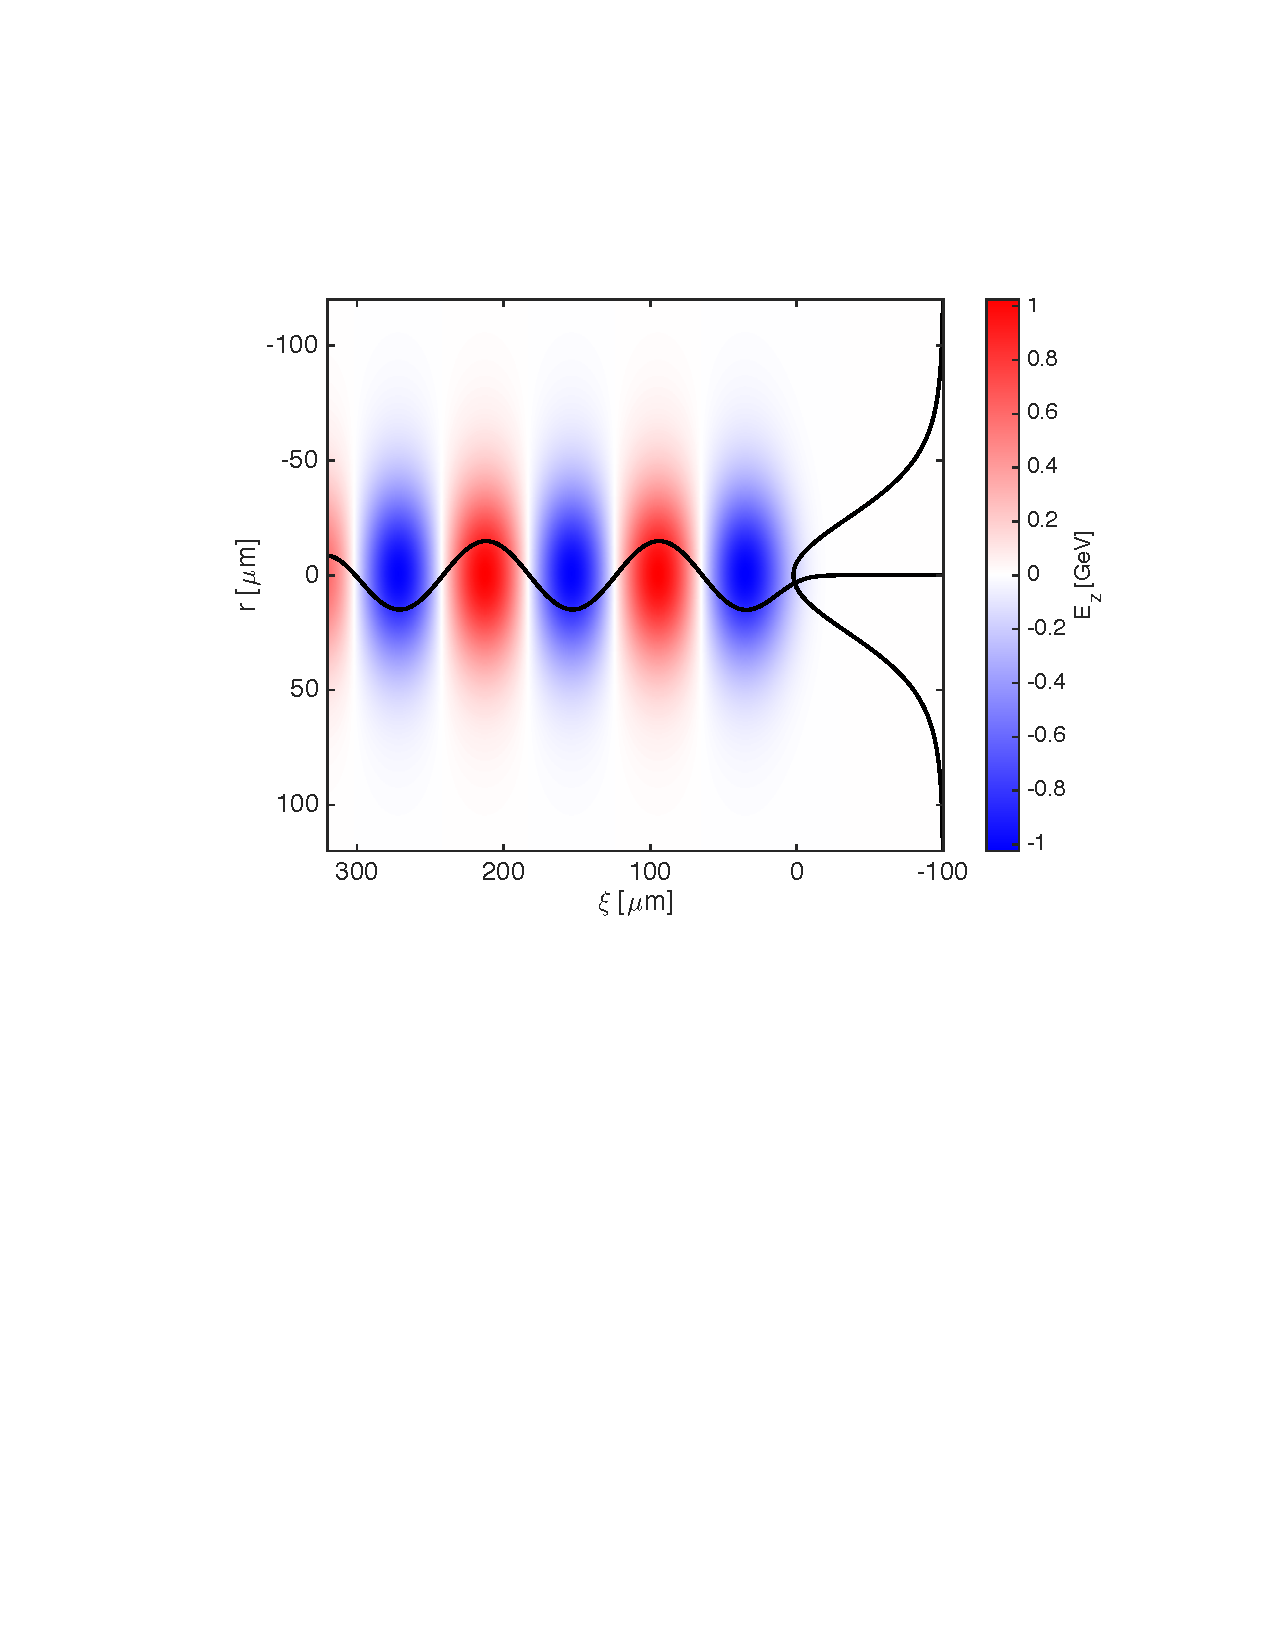
\includegraphics[width=0.49\textwidth]{longitudinal_gessner}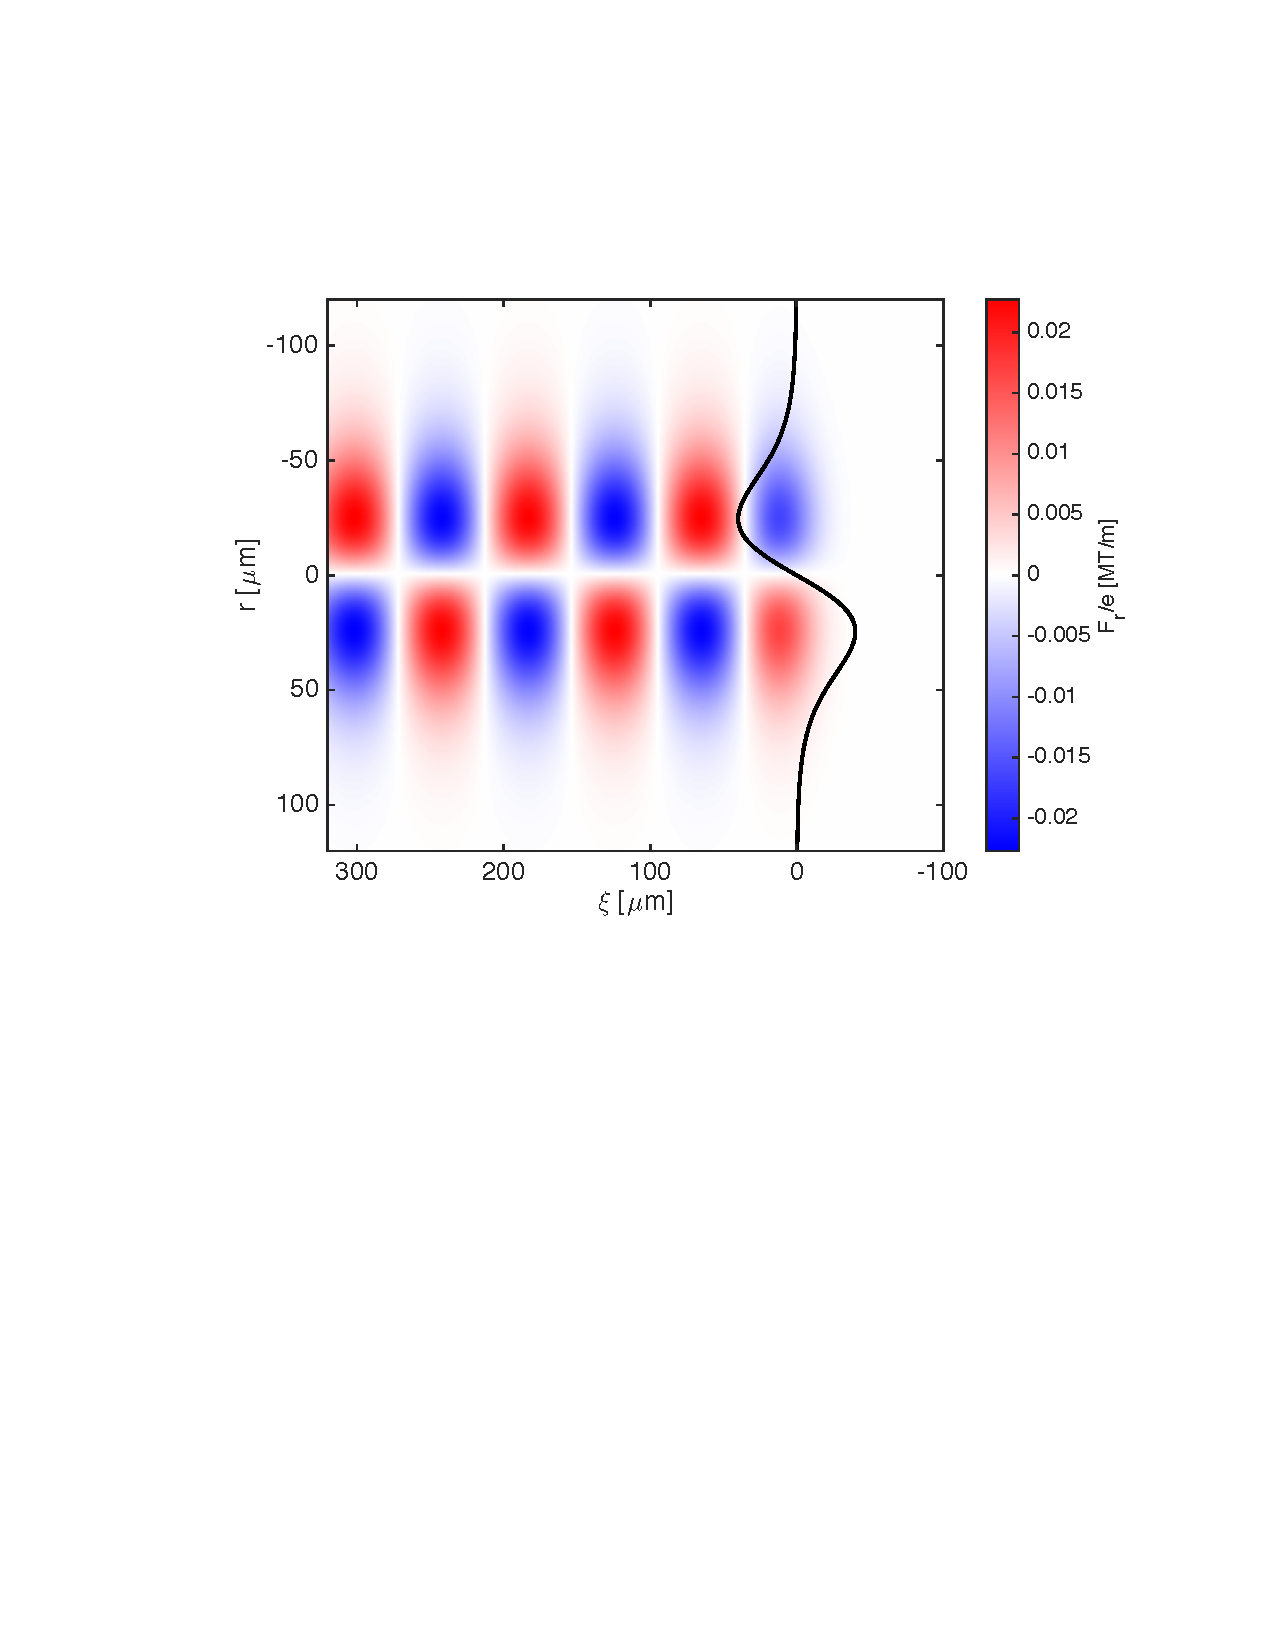
\includegraphics[width=0.49\textwidth]{transverse_gessner}
%\end{figure}
\begin{figure}
\centering
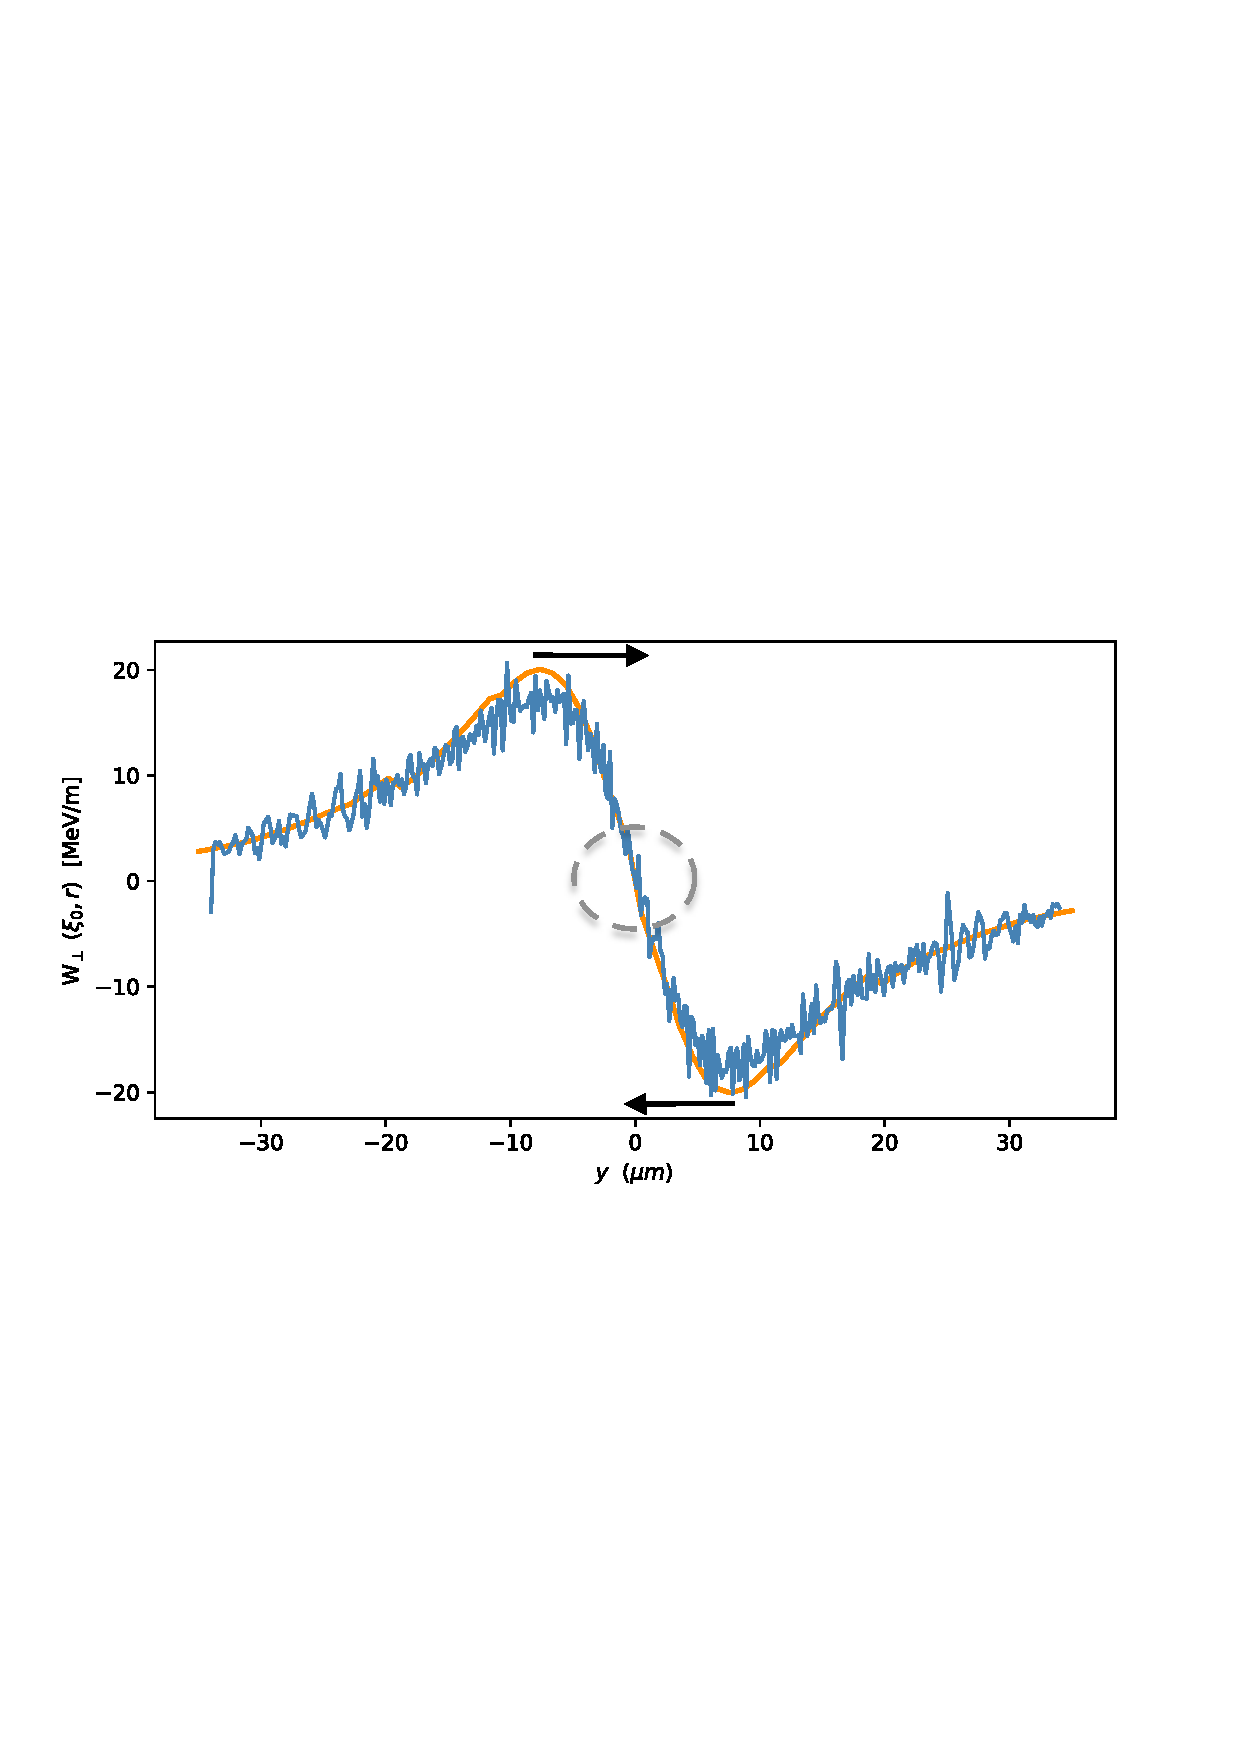
\includegraphics[width=\textwidth]{transverse_theory_vs_sim4.pdf}
\caption{Transverse force - theory vs. simulation}
\end{figure}

\subsection{Collective Plasma Deceleration -- Linear regime }
As described above parts of the electron bunch can be in either accelerating or decelerating regions. The parts of the bunch that are in a decelerating region will lose energy; this is the general idea behind a plasma beam dump. Since we can calculate the electric field at any position ($\xi,r$) along the bunch we can estimate the energy loss by calculating the work carried out by the longitudinal electric field. Since the beam is assumed to be rigid in the linear regime this does not take into account accelerated particles. This is the approach taken by Bonatto et al. to estimate the distance required to dump various beams in passive or active plasma beam dumps \citep{Bonatto2016}, and as we shall see in section XXX this approach provides good agreement with simulations.\\
The rate of energy change with propagation distance of a particle at position $(r,\xi)$ in the bunch after travelling is given by the force exerted on the particle by the longitudinal electric field:
\begin{equation}
\frac{\mathrm{d}U_p}{\mathrm{d}s}=-eE_z(r,\xi)
\end{equation}
where we have assumed that there occurs no modulation of the particle bunch as it traverses the plasma, hence the electric field is only a function of the position in the bunch $E_z(r,\xi)$ and not the propagation distance $s$. Integrating over the propagation distance then gives the energy of one particle in the beam at position $(r,\xi)$ after travelling a distance s:
\begin{equation}
U_e(r,\xi,s)=U_e(r,\xi,0)-seE_z(r,\xi)
\end{equation}
from which multiplication by the beam number density $n_b(r,\xi)$ and integration over the volume of the bunch gives the total energy of all particles in the bunch after propagation distance s
\begin{equation}
U(s)=\int  U_e(r,\xi,0)n_b(r,\xi)r\mathrm{d}r\mathrm{d}\xi\mathrm{d}\phi-se\int E_z(r,\xi)n_b(r,\xi)r\mathrm{d}r\mathrm{d}\xi\mathrm{d}\phi
\label{energy_loss_bonatto}
\end{equation}
where $E_z$ and $n_b$ are found from equations (\ref{longitudinalforce}) and (\ref{bigaussian}). A propgram to caluclate this numerically has not yet been implement, but we endevaour to do so in the second part of this project to allow for comaprisons between the linear theory with simulations and eventually with experiments at the FLASHForward facility at DESY.
%\subsection{Notes Bonatto}
%Rate of change due to the longitudinal electric field acting on an electron beam, i.e position beam in the decelerating region of the wakefield.\\
%"the beam only experiences its self-excited wakefield."\\
%In the passive beam dump, are we essentially slowing down a "drive bunch" without having a witness bunch behind to get accelerated?\\
%It is probaly better to u se gamma as in Bonatto's paper, to make it easier to explain total beam energy integral. Basically integrate over all particles.\\
%$U=\gamma m_ec^2$
%\begin{equation}
%-\frac{\mathrm{d}U}{\mathrm{d}s}=(F_e)_z=eE_z
%\end{equation}
%where $s$ is the distance travelled in the plasma and $U$ is the energy of a particle in the beam at position $\xi$. 
%for ultra relativistic beams, $\beta\sim 1$, the longitudinal electric field is a function of the position along the bunch $\xi=z-ct$ and not $z$ explicitly. 
%\begin{equation}
%U(s,\xi)=U_0-esE_z(\xi)
%\end{equation}
%The total energy of the beam after travelling a distance $s$ is then found by integrating across all the particles in the beam, which is integrating across $\xi$ since analysis is in 1-D.
%\begin{equation}
%\mathcal{U}(s)=U_0\int_{-\infty}
%\end{equation}

%We will proceed by calculating the gamma factor of a given particle in the beam who's energy we wish to compute.
%\begin{equation}
%\gamma(s,\xi)=\gamma_0-esE_z(\xi)
%\end{equation}

%Based on the work of Lu et. al \citep{Lu2006}, wherein it was shown that the predictions from the linear models perform well even in the non-linear regime, it is of interest to compute the energy loss in the linear regime. 

\section{Non-linear Regime} 
